\chapter{Compressed Sensing based Analog to Digital Converter}\label{C:cs-adc}

Traditional Nyquist Theory becomes cumbersome when an acquisition system processes wideband signals which contains a relatively high frequency component. In this chapter, we discuss  recent applications embedding CS into ADCs to reduce the sampling rate and improve ADCs’ performance. This chapter focuses on the CS based ADCs design, categories different popular CS-ADCs in areas of wireless communication, and finally discusses the architectures and compare the performance.

\section{Introduction}\label{ch3:intro}

Analog-to-Digital Converters (ADCs) are key components for signal acquisition and processing systems.
%%re-wr
Ideally, each sampling event should result in the signal value at the specific sampling instant. However, in practice, there are main factors that limit the ADC performance (e.g. increase system noise, phase offset and magnitude error, inter-symbol interference etc) such as uncertainty in the sampling instant (i.e., jitter) and the finite sampling bandwidth, manifested as a weighted integration over a small time interval around the sampling instant (i.e., aperture).
%%

What is worse, those effects become more serious at higher input signal frequencies, as the signal slew-rate (i.e., rate of change of a signal) is proportional to the signal frequency so that a small jitter or aperture uncertainty can generate non-idealities which cause a significant error in high-speed sampling, especially effects the performance in modern signal acquisition and processing systems which requires high frequency signal inputs.

The CS has enabled alternative solutions to this problem for high-speed ADCs in the area of CS based analog-information-convertion (AIC). Well-known applications of CS based AIC include random demodulator \cite{tropp2010beyond}, modulated wideband converter \cite{mishali2009blind} and non-uniform sampler \cite{ ragheb2007implementation}. It has been claimed that these AIC architectures enable high resolution at high frequencies while only using low frequency, which are sub-Nyquist ADCs. 

In addition, CS enable systems to acquire relatively small number of samples which reduce the power cost for sensing and storage. From these aspects, the CS based ADCs are important and needed to be investigated. 

\subsection{Sensing Matrix Modelling}
Since there is always not enough freedom for building random matrix (Gaussian or Bernoulli) subject to physical or other constraints in hardware implementations as well as the ADC designs, at the moment, the combination design comprised of partial randomness and partial deterministic (or termed as partial random structural matrix) becomes popular since most applications have constraints in design sensing matrix such as dictionary (Fourier basis) or channel impulse response, although many those combination design cannot reach the optimal boundary of minimum required samples $O(k log(\frac{N}{k}))$. In the following CS-ADC applications, most of the sensing matrices that are partial random structural matrices are analysed in their sub-section named \emph{Acquisition Model}, and corresponding reconstruction performances (in terms of sampling rates / minimum required samples) are displayed in sub-section named \emph{Fast Reconstruction}. 

\section{Random Demodulator}

Random Demodulator (RD) \cite{tropp2010beyond} is a newer and more popular ADCs for CS-based signal acquisition and processing.

\begin{figure}[!t]
\centering
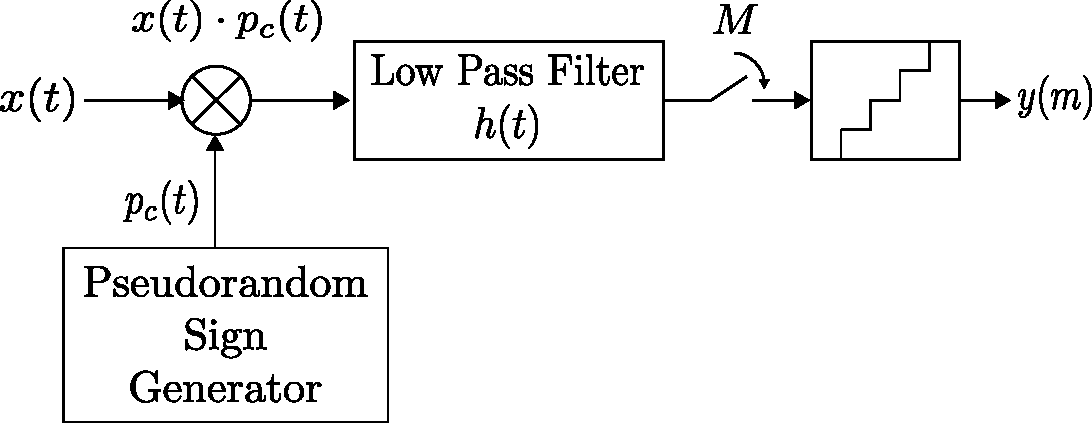
\includegraphics[width=0.5\columnwidth]{random_demodulator.pdf}
\DeclareGraphicsExtensions.
\caption{Block diagram of random demodulator (RD). The components includes a pseudo-random sign generator, a low-pass filter, and a sub-Nyquist ADC}\label{RD}
\end{figure}

The k-sparse input signal x is first mixed with the chipping sequence $p_c(t)$ which is a waveform constructed by pseudo-random variables of $\{\pm 1\}$ (termed as chipping sequence). The mixed product component $x(t) \cdot p_c(t)$ is then passed through an anti-aliasing low pass filter $h(t)$, before being sampled at a uniform interval but at a lower sampling rate of $m$ which is of the order $O(K log(N/K))$ which is much lower than the normal required rate corresponds to $N$ (since $K << N$). The most widely used reconstruction algorithms for RD are those based on OMP and CoSaMP greedy pursuit. Experimental results \cite{tropp2010beyond} demonstrates that the minimal sampling rate needed is only $1.7K(log(N/K))$ and in addition, it provides better SNR performance when compared with conventional Nyquist rate based ADCs.

\subsection{Acquisition Model}

We first assume the RD acting on the discrete time domain instead of the continuous-time domain. We first suppose $x = \Psi s$, where $\Psi$ is the discrete time Fourier transform (DFT) matrix and $s$ is $K$ sparse coefficients. Next, the RD measurement $\Phi$ can be described as a combination of two matrices representing chipping sequence $p_c(n)$ and sub-Nyquist sampling action, respectively.

First, we consider the action of mixing chipping sequence $p_c(n)$ described as diagonal matrix $D$ where the value $\epsilon$ of non-zero items (diagonal items) are chosen pseudo-randomly from the set $\{-1,+1\}$ as shown in (\ref{mx_chipping}):
\begin{equation}
\label{mx_chipping}
D = \left(
\begin{array}[c]{cccc}
\epsilon_0 & & &\\
& \epsilon_1 & &\\
& & \ddots &\\
& & &\epsilon_{n-1}
\end{array}\right)_{N \times N}
\end{equation}

Next, we consider the action of the sampling at a sub-Nyquist rate $M$. Suppose that $M$ divides the Nyquist rate $N$, then each sample is the sum of $N/M$ consecutive entries of input signal\cite{kirolos2006analog}. In summary, this sampling behaviour can be treated as an $M \times N$ matrix $\Phi$ in (\ref{mx_subsample}) where each row has $N/M$ successive entries beginning with its $mN/M+1$ th item, where $m = 0,1,\ldots, N-1$ refers to the column number.

\begin{equation}
\label{mx_subsample}
\Phi = \left(
\begin{array}[c]{cccc}
{\underbrace{{1\hspace{0.15em}1}\ldots 1 }_{N/M}}& & & \\
 & {{1\hspace{0.15em}1}\ldots 1 } & & \\
 & & \ddots & \\
 & & & {{1\hspace{0.15em}1}\ldots 1 }
\end{array}\right)_{M \times N}
\end{equation}

In conclusion, the final observation behaviour of RD can be modernised as the following (\ref{mx_measure}),
\begin{equation} 
\label{mx_measure}
y = (\Phi D) x = (\Phi D \Psi) s = As
\end{equation}
where $\Phi D$ stands for the architecture in Figure \ref{RD} and $A$ is the final measurement for sparse components $s$, providing stable and robust reconstruction if $A$ satisfies the RIP.

\subsection{Fast Reconstruction}

Convex optimisation and greedy pursuits have been both developed and applied in this architecture such as OMP and CoSaMP, and they have been widely used for reconstruction for RD \cite{yang2009compressed,bai2012high}. According to experimental results of RD\cite{tropp2010beyond}, the necessary minimal samples for stable reconstruction for this architecture is $1.7K(\log(N/K))+1$ and similar to the theoretical results\cite{donoho2006high} stating the theorcial minimum number in compressive sampling using random matrix. Hence, the required samples for CS reseaches a magnitude of $OK(\log(N/K))$ ($K << N$) and considered much less than $2N$ samples needed for Nyquist sampling. Besides,\cite{tropp2010beyond} also find out that the robustness of RD surpasses that of the traditional Nyquist sampling by testing of the signal-to-noise ratio (SNR) in different situations.

\section{Modulated Wideband Convertor}

Modulated Wideband Converter (MWC) \cite{mishali2009blind} is an approach that applies the CS theory for traditional blind multi-band signal receivers \cite{black1980time}, where the carrier frequency is either time-variant or unknown. Figure \ref{MWC1} shows the architecture of the MWC, which consists of parallel channels of RD based sub-Nyquist rate ADCs.

Each periodic sequence (at $T_P$ interval) of $p_i(t)$ with minimum duration of $T_p/M$ is mixed with the input multi-band signal $x(t)$. This shifts each channel spectrum by $\Delta f_p$ ($f_p = 1/{T_p}$ which is then filtered to the baseband for sampling by sub-Nyquist ADCs. Reconstruction is done by support detection via continuous to finite block (CTF) which is shown in Figure \ref{ctf}, and the followed signal reconstruction, where the CTF block is comprised of frame construction and the multiple measurement vectors (MMV) reconstruction, and the signal reconstruction can be achieved by a direct pseudo-inverse operation based on results of the CTF block.

\begin{figure}[!t]
\centering
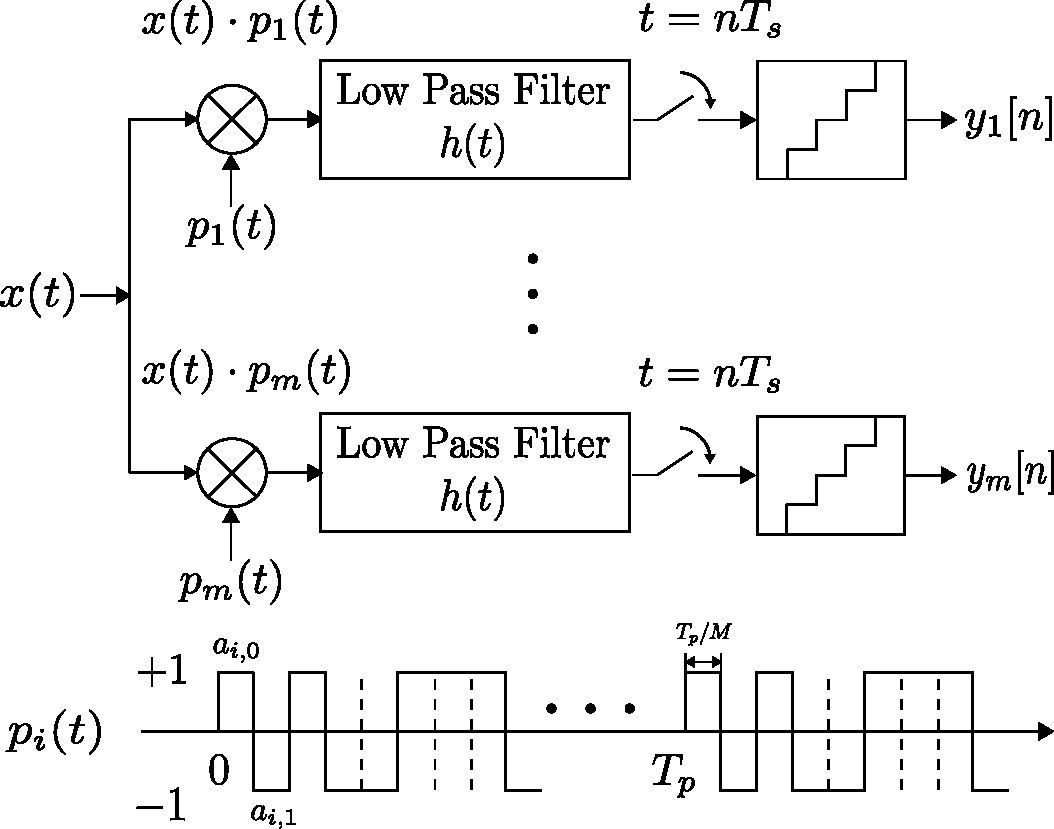
\includegraphics[width=0.5\columnwidth]{MWC1.pdf}
\DeclareGraphicsExtensions.
\caption{Block diagram of modulated wideband convertor (MWC). The components includes parallel periodic waveforms mixers, low-pass filters, and sub-Nyquist ADCs}\label{MWC1}
\end{figure}

\subsection{Acquisition Model}

We assume that MWC samples a multi-band signal $x(t)$ obtaining sparse spectrum $X(f)$ supported by N frequency segments (Each of segments does not exceed B Hz). When $x(t)$ is mixed by the $p_i(t)$
%a periodic piecewise sequence $p_i(t)$ which alternates between $\pm1$ at time interval $T_p/M$ and chipping sequence in \ref{RD} can be used.
the spectrum $X(f)$ of $x(t)$ becomes: 
\begin{equation}
\label{eqn_mwc1}
\begin{split}
\begin{aligned}
\bar X_i(f) = \int_{-\infty}^{+\infty} x(t) p_i(t) e^{-j2\pi ft}dt \\
= \sum_{l=-\infty}^{+\infty} c_{il} X(f-lf_p)
\end{aligned}
\end{split}
\end{equation}
, where the periodic sequence $p_i(t)$ can be represented by:
\begin{equation}
\label{eqn_mwc2}
p_i(t)=\sum_{l=-\infty}^{+\infty}c_{il}e^{j\frac{2\pi}{T_p}lt},\; c_{il}= \frac{1}{T_p}\int_{0}^{T_p}p_i(t)e^{j\frac{2\pi}{T_p} lt} dt
\end{equation}
\begin{figure}[!t]
\centering
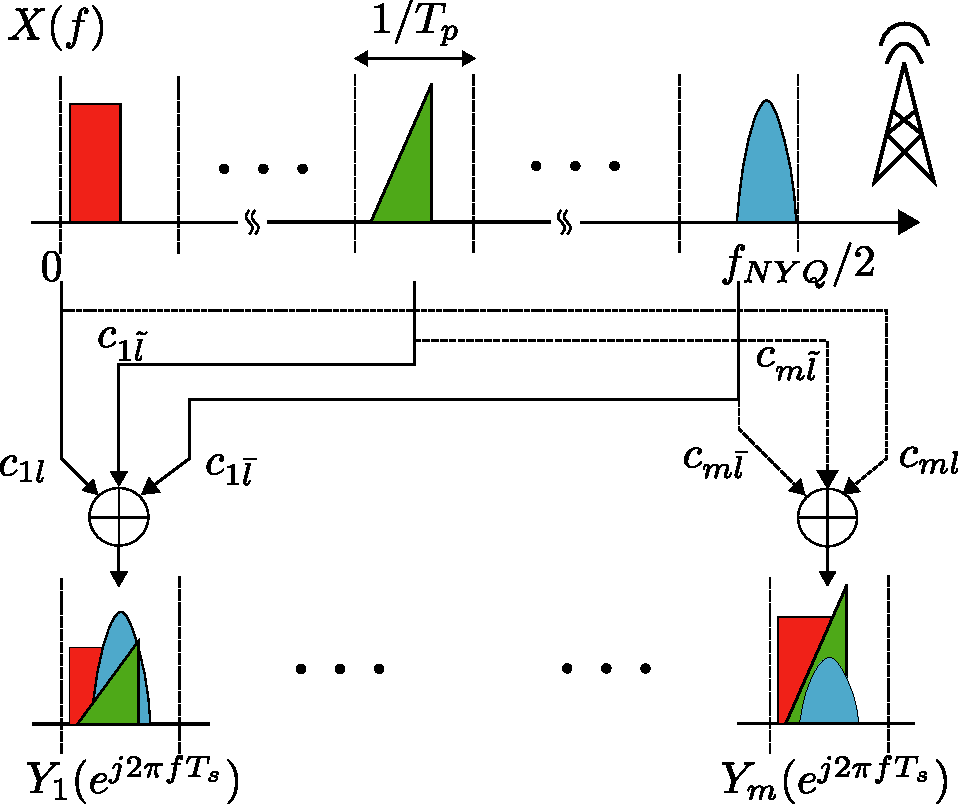
\includegraphics[width=0.5\columnwidth]{MWC2.pdf}
\DeclareGraphicsExtensions.
\caption{
Block diagram of the relationship between the spectrum of the output $y_i(n)$ and the input $X(f)$ In this example, channels $1$ and $m$ linearly combines the original the spectrum segments around $lf_p$, $\bar lf_p$, $\tilde lf_p$ with different weights $c_{il}$.
}\label{MWC2}
\end{figure}

Sampled to baseband by filters and ADCs, the weighted and accumulated $X(f)$ has a relationship with the discrete-time Fourier transform (DTFT) of $y_i[n]$ (the $ith$ group of the output) shown in (\ref{eqn_mwc3}):
\begin{equation}
\label{eqn_mwc3}
Y_i(e^{j2\pi fT_s})=\sum_{l=-L_0}^{+L_0}c_{il}X(f-lf_p)
\end{equation}
, where $T_s = 1/{f_s}$, and $L0$ satisfies $2(L_0+1)f_p \geq f_{NYQ}+f_s$ and $2L_0+1=M$.

Since (\ref{eqn_mwc3}) establishes the relationship between observations and input sparse signals, the measurement or the CS sensing matrix can be described as $\mathbf y(f) = C \mathbf z(f)$:
\begin{align}
\label{eqn_mwc4}
\underbrace{\left[\small
\begin{array}[c]{c}
Y_1(e^{j2\pi fT_s}) \\
\vdots  \\
Y_m(e^{j2\pi fT_s})
\end{array}
\right]}_{\mathbf y(f)} =
\underbrace{\left(\small
\begin{array}[c]{ccc}
 c_{11} & \ldots & c_{1M} \\
 \vdots &  \ddots & \vdots\\   
 c_{m1}& \ldots & c_{mM}
\end{array}
\right)}_{C}
\underbrace{\left[\small
\begin{array}[c]{c}
X(f-{L_0}f_p) \\
\vdots  \\
X(f+{L_0}f_p)
\end{array}
\right]}_{\mathbf z(f)}
\end{align}
, where $C = \{c_{il}\}_{m \times M}$ depends on the choice of different $p_i(t)$. A popular application of $p_i(t)$ is referred as the sign waveform generator in RD\cite{mishali2010theory} as well as in Figure \ref{MWC1}, produced by a shift-register structure. In this case, the corresponding coefficients $c_{il}$ equals:
\begin{equation}
\begin{split}
\begin{aligned}
c_{il}= \frac{1}{T_p} \int_{l=0}^{\frac{T_p}{M}} \sum_{k=0}^{M-1} a_{ik} e^{j \frac{2\pi}{T_p} l (t+k \frac{T_p}{M})} \\
      = \frac{1}{T_p} \sum_{k=0}^{M-1} a_{ik} e^{-j \frac{2\pi}{M} lk } \int_{l=0}^{\frac{T_p}{M}} e^{-j \frac{2\pi}{M} lt }
\end{aligned}
\end{split}
\label{eqn_mwc5}
\end{equation}
, where $a_{m,M-1} \in \{\pm1\}$ refers to the value of the $p_i(t)$. Embedding the presentation of $c_{il}$ to the (\ref{eqn_mwc4}), the CS sensing matrix of the MWC can be represented as: $Y_i(e^{j2\pi fT_s})= CX(f) = HFDX(f)$, where $C$ consists of $HFD$ as follows:
\begin{align}
\label{eqn_mwc6}
\underbrace{\left(\footnotesize
\begin{array}[c]{ccc}
a_{1,0}&\ldots &a_{1,M-1} \\
\vdots &\ddots & \vdots \\
a_{m,0}&\ldots &a_{m,M-1}
\end{array}\right)}_{H_{m \times M}}
\underbrace{\left(\small
\begin{array}[c]{ccc}
| & \ldots & | \\
\bar F_{L_0} & \ldots &  \bar F_{-L_0}\\   
| & \ldots & |
\end{array}\right)}_{F_{M \times M}}
\underbrace{\left(\footnotesize
\begin{array}[c]{ccc}
d_{0}&& \\
&\ddots &  \\
&&d_{M-1}   
\end{array}\right)}_{D_{M \times M}}
\end{align}
, where $F$ is the discrete time Fourier transform (DFT) matrix constructed by $\bar F_{L_i} = [e^{-j0\cdot i},\ldots, e^{-j \frac{2\pi}{M} (M-1)\cdot i}]$ and $D = \{d_l = \frac{1}{T_p} \int_{0}^{\frac{T_p}{M}} e^{-j \frac{2\pi}{M} lk}\}$.

\subsection{Fast Reconstruction}

Considering the CS measurement in (\ref{eqn_mwc4}), recovering the $\mathbf z(f)$ where each row $X(f-lf_p)$ presents sparse spectrum segments can be regarded as recovering a infinite set of joint sparse vectors. This problem can be solved by changing it to the problem of multiple measurement vectors (MMV)\cite{mishali2008reduce} and has been implemented as Figure \ref{ctf}:

Step 1: Calculating $Q = \sum_{-\infty}^{+\infty}\mathbf y[n]\mathbf y^{T}[n]$, where $\mathbf y[n]$ = $[y_1[n],\ldots,y_m[n]]^{T}$ is the output sampled at the time interval $nT_s$. Then finding the matrix $V$ by solving $Q = VV^T$.

Step 2: After gain $V$, solving the MMV problem defined as $V = CU$, where $C$ refers to the measurement of MWC in (\ref{eqn_mwc4}) and (\ref{eqn_mwc6}). Since applying the chipping sequence in RD \cite{mishali2010theory} as $p_i(t)$ for MWC is proven applicable and satisfied the expected RIP \cite{mishali2009expected}, the matrix $C$ has sufficient guarantees to provide stable and robust reconstructions for MMV based $l1$-minimisation\cite{mishali2008reduce}, changing this HP-hard problem to a polynomial time computable. Furthermore, MMV greedy pursuits  in\cite{chen2006theoretical,mishali2008reduce,sun2009efficient} presents better computational performance and widely used. Then the joint sparse $\Omega$ is recovered as $\Omega = \cup_{i \in \Omega} supp(U)$.

Since MWC in Figure \ref{MWC1} satisfies the expected RIP \cite{mishali2009expected}, the problem of multiple measurement vectors (MMV) can solved in CS theory. Hence the above procedures finally  recovers the input infinite set $\Omega$ of joint sparse vectors $\mathbf z(f)={X(f-lf_p)}$, and use $\mathbf z(f)$ recover the $x[n_{Ts}]$, the recovery of the blind multi-band signal in time domain:
\begin{equation}
\label{eqn_zn}
z[n] = C_{\Omega}^{\dagger} y[n], \quad C_{\Omega}^{\dagger} = C_{\Omega}^T(C_{\Omega}^TC_{\Omega})^{-1}C_{\Omega}
\end{equation}
, where C is the matrix in (\ref{mx_measure}) and $\mathbf z[n]$ is the set of the inverse DTFT of $z_i[f] = X(f-lfp)$ in (\ref{eqn_mwc4}). Hence, $x(nT_s)$ can be generated by shifting spectrum slice $z_i(f)$ to appropriate position using a low pass filter $h_{LP}(n)$, and summing up them with zero padding\cite{mishali2010theory}:
\begin{equation}
x[n]=x[n_{Ts}]=\sum_{i\in\Omega} (z_i[n]*h_{LP}[n])e^{2\pi if_pnT}
\end{equation}
\begin{figure}[!t]
\centering
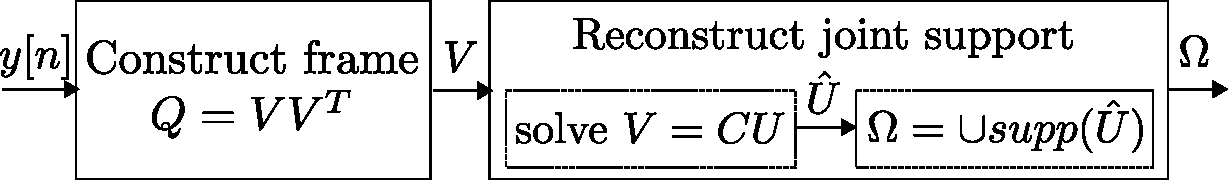
\includegraphics[width=0.5\columnwidth]{ctf.pdf}
\DeclareGraphicsExtensions.
\caption{Block diagram of Continuous to Finite (CTF) for the joint supports detection}\label{ctf}
\end{figure}
\quad  As a result, in practical applications the experimental results indicates that stable recovery of the MWC in Figure \ref{MWC1} requires roughly $m \approx 4Nlog(M/2N)$ channels to estimate the correct support.

Moreover, the comparison of a modulated wide-band converter(MWC) and a random demodulator(RD) is provided in \cite{mishali2011xamplingsignal} from aspects of hardware complexity, robustness and computational load. As shown in experimental results, the two structure contains the similar hardware complexity, but the MWC outperforms the RD in computational load and robustness to model mismatch\cite{mishali2011xamplingsignal}.

\section{Non-Uniform Sampling}

Apart from the modulated based CS architectures such as random demodulators (RD) or modulated wideband converters (MWC) which uniformly samples the mixed input analog signals at a slow rate, another novel CS architecture is the non-uniform sampling (NUS), based on the theory of information recovery from random samples \cite{ragheb2007implementation}, is driven by a pseudo random clock that produce a sub-Nyquist rate on average. An example of this sampling pattern is shown in Figure \ref{RS-ADC}, and an instance of NUS application implemented by multiplexers is shown in Figure \ref{RS-ADC}.

\begin{figure}[!t]
\centering
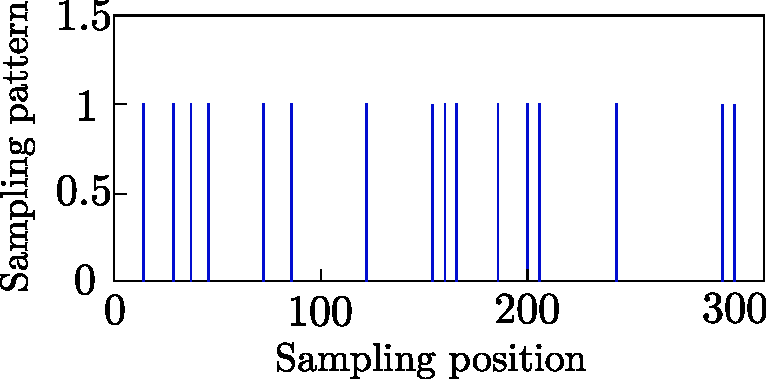
\includegraphics[width=0.5\columnwidth]{NUS.pdf}
\DeclareGraphicsExtensions.
\caption{A pseudo-randomly sample pattern for single pure tone signal of length 300}\label{NUS}
\end{figure}

\subsubsection{Acquisition Model and Reconstruction}

Considering randomly reducing the number of measurements make the signal $x$ under-sampled with a low average sampling rate, we presents the behaviour of the non-uniform sampler (NUS)\cite{candes2008introduction} based CS acquisition model can be represented as a matrix representation:
\begin{align}
\label{non-uniform_sample3}
\left[
\begin{array}[c]{c}
| \\
y  \\
|
\end{array}
\right] =
\underbrace{\left(
\begin{array}[c]{ccc}
\epsilon_0 && \\
&\ddots &  \\
&&\epsilon_{n-1}
\end{array}\right)}_{D_{N \times N}}
\underbrace{\left(
\begin{array}[c]{ccc}
1 & \ldots & \omega^{0 \cdot (N-1)} \\
\vdots & \ddots & \vdots  \\   
1 & \ldots & \omega^{(N-1)(N-1)}
\end{array}\right)}_{F_{N \times N}}
\left[
\begin{array}[c]{c}
| \\
s  \\
|
\end{array}
\right]
\end{align}
, where the matrix multiplication between $F$ and $s$ stands for the input signal $x$ which contains sparse spectrum $s$, and $F$ is the full discrete time Fourier transform (DFT) matrix. The diagonal matrix $D$ represents the behaviour of non-uniform sampling, where the value $\epsilon$ of diagonal items are chosen pseudo-randomly from $\{0,1\}$.

The NUS based CS acquisition model establishes a sensing matrix $A$ which equal $DF$ in \ref{non-uniform_sample3} and can be regarded as a random partial Fourier matrix $F_{T}$ which consists of randomly chosen columns of the discrete Fourier matrix(DFT) and indexed by $T$. According to \cite{ragheb2007implementation}, the matrix $A$ satisfies the RIP in compressive sensing so the acquisition model in (\ref{non-uniform_sample3}) produces a stable reconstruction of $\hat s$ via $l1$-minimisation using $m \geq O(slog(N/s))$ samples\cite{ragheb2007implementation}. In addition, many greedy algorithms such as OMP and CoSaMP are also implemented as fast reconstruction for this architecture\cite{maechler2011random}.

\subsubsection{Implementation}

Common implementations of the CS based non-uniform sampling architectures varies from \cite{laska2006random, ragheb2007implementation, maechler2011random, rogers2011compressive}. Among these implementations, the random sampling compressive sensing ADC (RS-ADC) is likely to be the prevailing design shown in Figure \ref{RS-ADC}. The implementation uses an input multiplexer driven by a non-uniform clock to switch the signal among several parallel $S/H$ based analog queues. A low rate ADC (e.g. Successive Approximation ADC) is used to convert the stored samples, performing at uniform intervals but operating at sub-Nyquist average rate. Greedy pursuit algorithms such as OMP and CoSaMP are then used to perform fast reconstruction for this architecture.

\begin{figure}[!t]
\centering
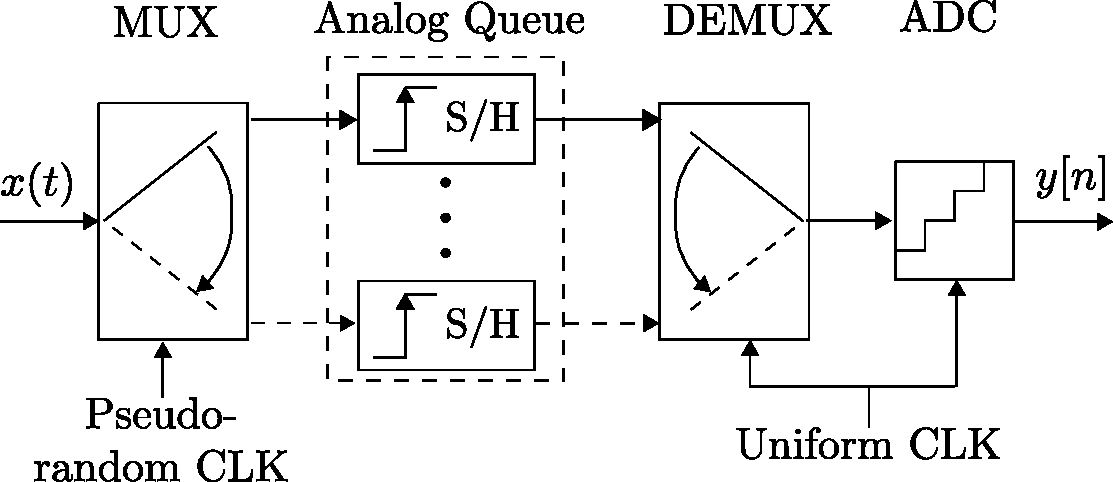
\includegraphics[width=0.5\columnwidth]{RSADC.pdf}
\DeclareGraphicsExtensions.
\caption{Block diagram of the random sampling CS ADC (RS-ADC). The components includes a pseudo-random sign generator, a low-pass filter, and a sub-Nyquist ADC}\label{RS-ADC}
\end{figure}

However, the main problem of applying RS-ADC lies in sampling high frequency signals: since the ADC and input MUX perform inherent bandwidth limitations modeled as a lowpass filter preceding the uniform sampling, acquisitions for high frequency signals results in a loss of the spectrum components. Besides, the high switching speed of the MUX increases noise and reduces the power efficiency.

\section{Conclusion}

Modern digital signal processing applications deal with a large amount of data, resulting in enormous numbers of observations and requiring high speed sampling in the front-end of systems according to the Nyquist theorem. To overcome this problem, the compressive sensing based ADC (CS-ADC) is studied recently, and in this chapter, we provide a comprehensive survey of the novel CS-ADC designs in terms of architectures. We have traced origins of this technology and presented mathematical and theoretical foundations, as well as implementation instances including RD, MWC, and NUS. Reconstruction performance are discussed, which shows the computational efficiency and high speeds are achieved in CS-ADCs. Consequently, CS-ADCs become widely applied as sampling front-ends in many high frequency signal or wideband signal processing systems in many wireless devices such as ultra-wideband communications and cognitive radios that we will mentioned as our CS applications in the following chapters.  

%\subsection{Related Work}
%\subsection{random convolution} //OK
%As \ref{RD}, when we treated the RD in frequency domain, the sampling behaviour can be ($i$) convoluting sparse signal with pseudo-random chipping sequence and ($ii$) filtering the output by a low pass filter. This is the architecture of random convolution (RC)[]. Hence from this aspect, RD would be very similar to RC.
%\subsection{sublinear FFT} //OK
%In addition, instead of using uniform sub-Nyquist ADC, the algorithm termed sub-linear FFT suggests that one can subsample at a small number of random time from a structured grid. This method avoid jitters from non-uniform sampling and achieve average rate that is significantly lower than the Nyquist rate. This idea is implemented in [][], and will be introduced in the following section of $random\; sampling$.
%The use of Toeplitz matrices in CS applications has several potential advantages: (i) they require the generation of only O(n) independent random variables; (ii) multiplication with Toeplitz matrices can be efficiently implemented using fast Fourier transform, resulting in faster acquisition and reconstruction algorithms; and (iii) Toeplitz-structured matrices arise naturally in certain application areas such as system identification\cite{bajwa2007toeplitz}
